\documentclass[border=4pt]{standalone}
% Shared typography and colours for the standalone figures.
\usepackage{unicode-math}
\setmainfont{TeX Gyre Termes}
\setmathfont{TeX Gyre Termes Math}
\usepackage{tikz}
\usetikzlibrary{arrows.meta,positioning,calc,decorations.pathreplacing}
\usepackage{pgfplots}
\pgfplotsset{compat=1.18}
% Stored subsystem, transfer channel, driver, and internal observation.
\definecolor{elemA}{HTML}{1F5FA8}
\definecolor{elemB}{HTML}{B8461B}
\definecolor{elemC}{HTML}{2E7D32}
\definecolor{elemD}{HTML}{6A4C93}
\definecolor{frameline}{HTML}{555555}

\begin{document}
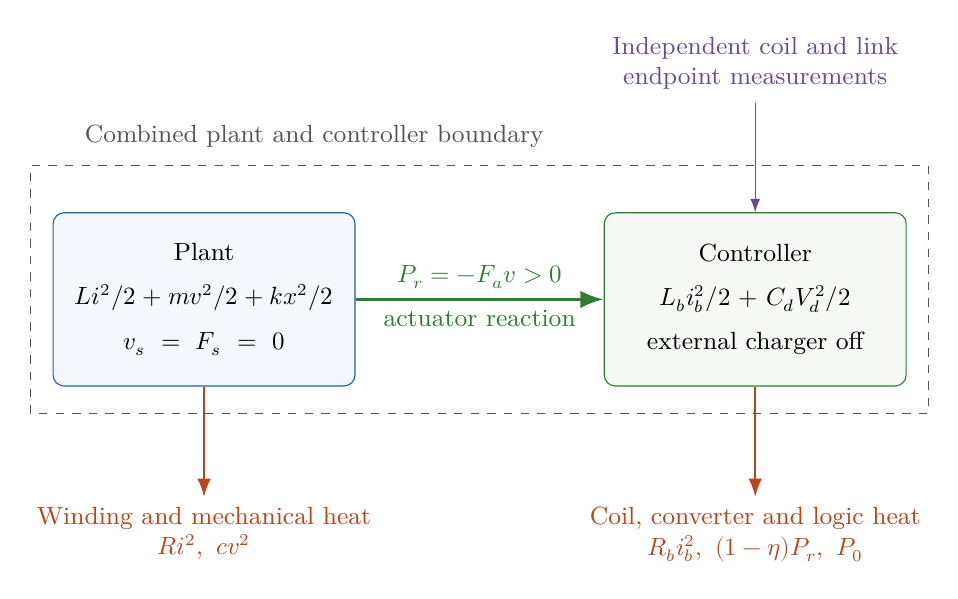
\begin{tikzpicture}[>=Latex,font=\small,
 box/.style={draw,rounded corners,align=center,minimum height=2.2cm,text width=3.6cm}]
\node[box,draw=elemA,fill=elemA!5] (plant) at (0,0) {Plant\\[5pt] $Li^2/2+mv^2/2+kx^2/2$\\[5pt] $v_s=F_s=0$};
\node[box,draw=elemC,fill=elemC!5] (ctrl) at (7,0) {Controller\\[5pt] $L_bi_b^2/2+C_dV_d^2/2$\\[5pt] external charger off};
\draw[->,very thick,elemC] (plant.east) -- node[above] {$P_r=-F_av>0$} node[below] {actuator reaction} (ctrl.west);
\draw[->,thick,elemB] (plant.south) -- ++(0,-1.4) node[below,align=center] {Winding and mechanical heat\\ $Ri^2,\ cv^2$};
\draw[->,thick,elemB] (ctrl.south) -- ++(0,-1.4) node[below,align=center] {Coil, converter and logic heat\\ $R_bi_b^2,\ (1-\eta)P_r,\ P_0$};
\draw[dashed,frameline] (-2.2,-1.45) rectangle (9.2,1.7);
\node[anchor=south,frameline] at (1.4,1.8) {Combined plant and controller boundary};
\node[elemD,align=center] at (7,3) {Independent coil and link\\ endpoint measurements};
\draw[->,elemD] (7,2.5) -- (ctrl.north);
\end{tikzpicture}
\end{document}
